\begin{frame}{Affirmation et négation}
  Quelle est la bonne conjugation? \\
  \tinygloss{What is the correct conjugation?}
  \begin{columns}
    \column{0.5\textwidth}
      \begin{enumerate}
        \item J'\underline{\uncover<2->{invite}} (inviter) mes parents.
        \item On ne \underline{\uncover<4->{regarde}} (regarder) pas la télé.
        \item Elle n'\underline{\uncover<6->{aime}} (aimer) pas le tennis.
        \item Ils \underline{\uncover<8->{habitent}} (habiter) à la maison.
        \item Nous \underline{\uncover<10->{retrouvons}} (retrouver) nos amis.
        \item Vous ne \underline{\uncover<12->{travaillez}} (travailler) pas au restaurant.
      \end{enumerate}
    \column{0.5\textwidth}
      \begin{minipage}[c][0.6\textheight]{\linewidth}
        \begin{center}
          \only<1-2>{
            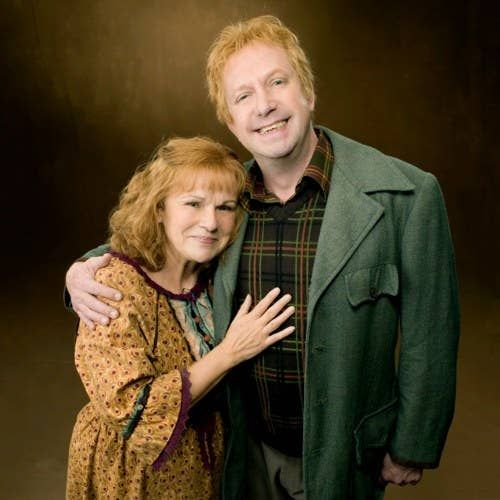
\includegraphics[scale=0.3]{weasley.jpg}
          }
          \only<3-4>{
            
\includegraphics[scale=0.09]{television.jpg}
          }
          \only<5-6>{
            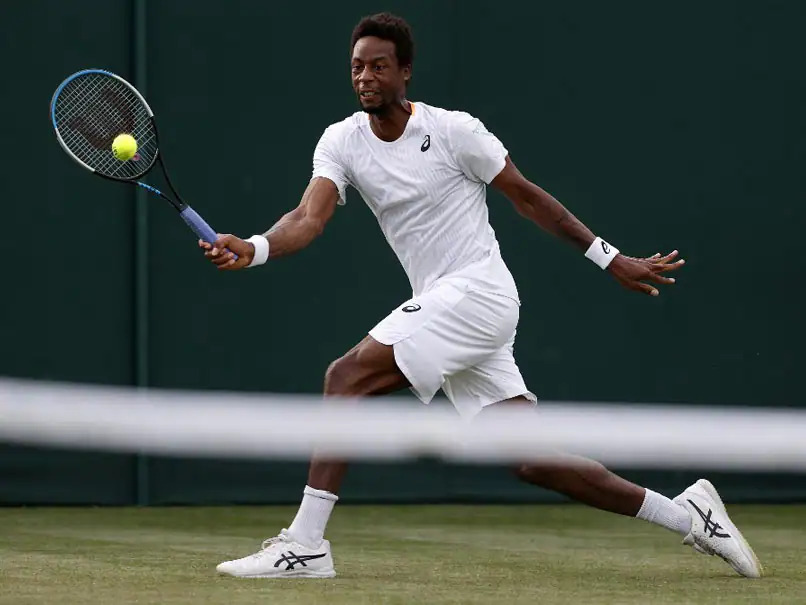
\includegraphics[scale=0.2]{monfils.jpg} \\
            Gaël Monfils
          }
          \only<7-8>{
            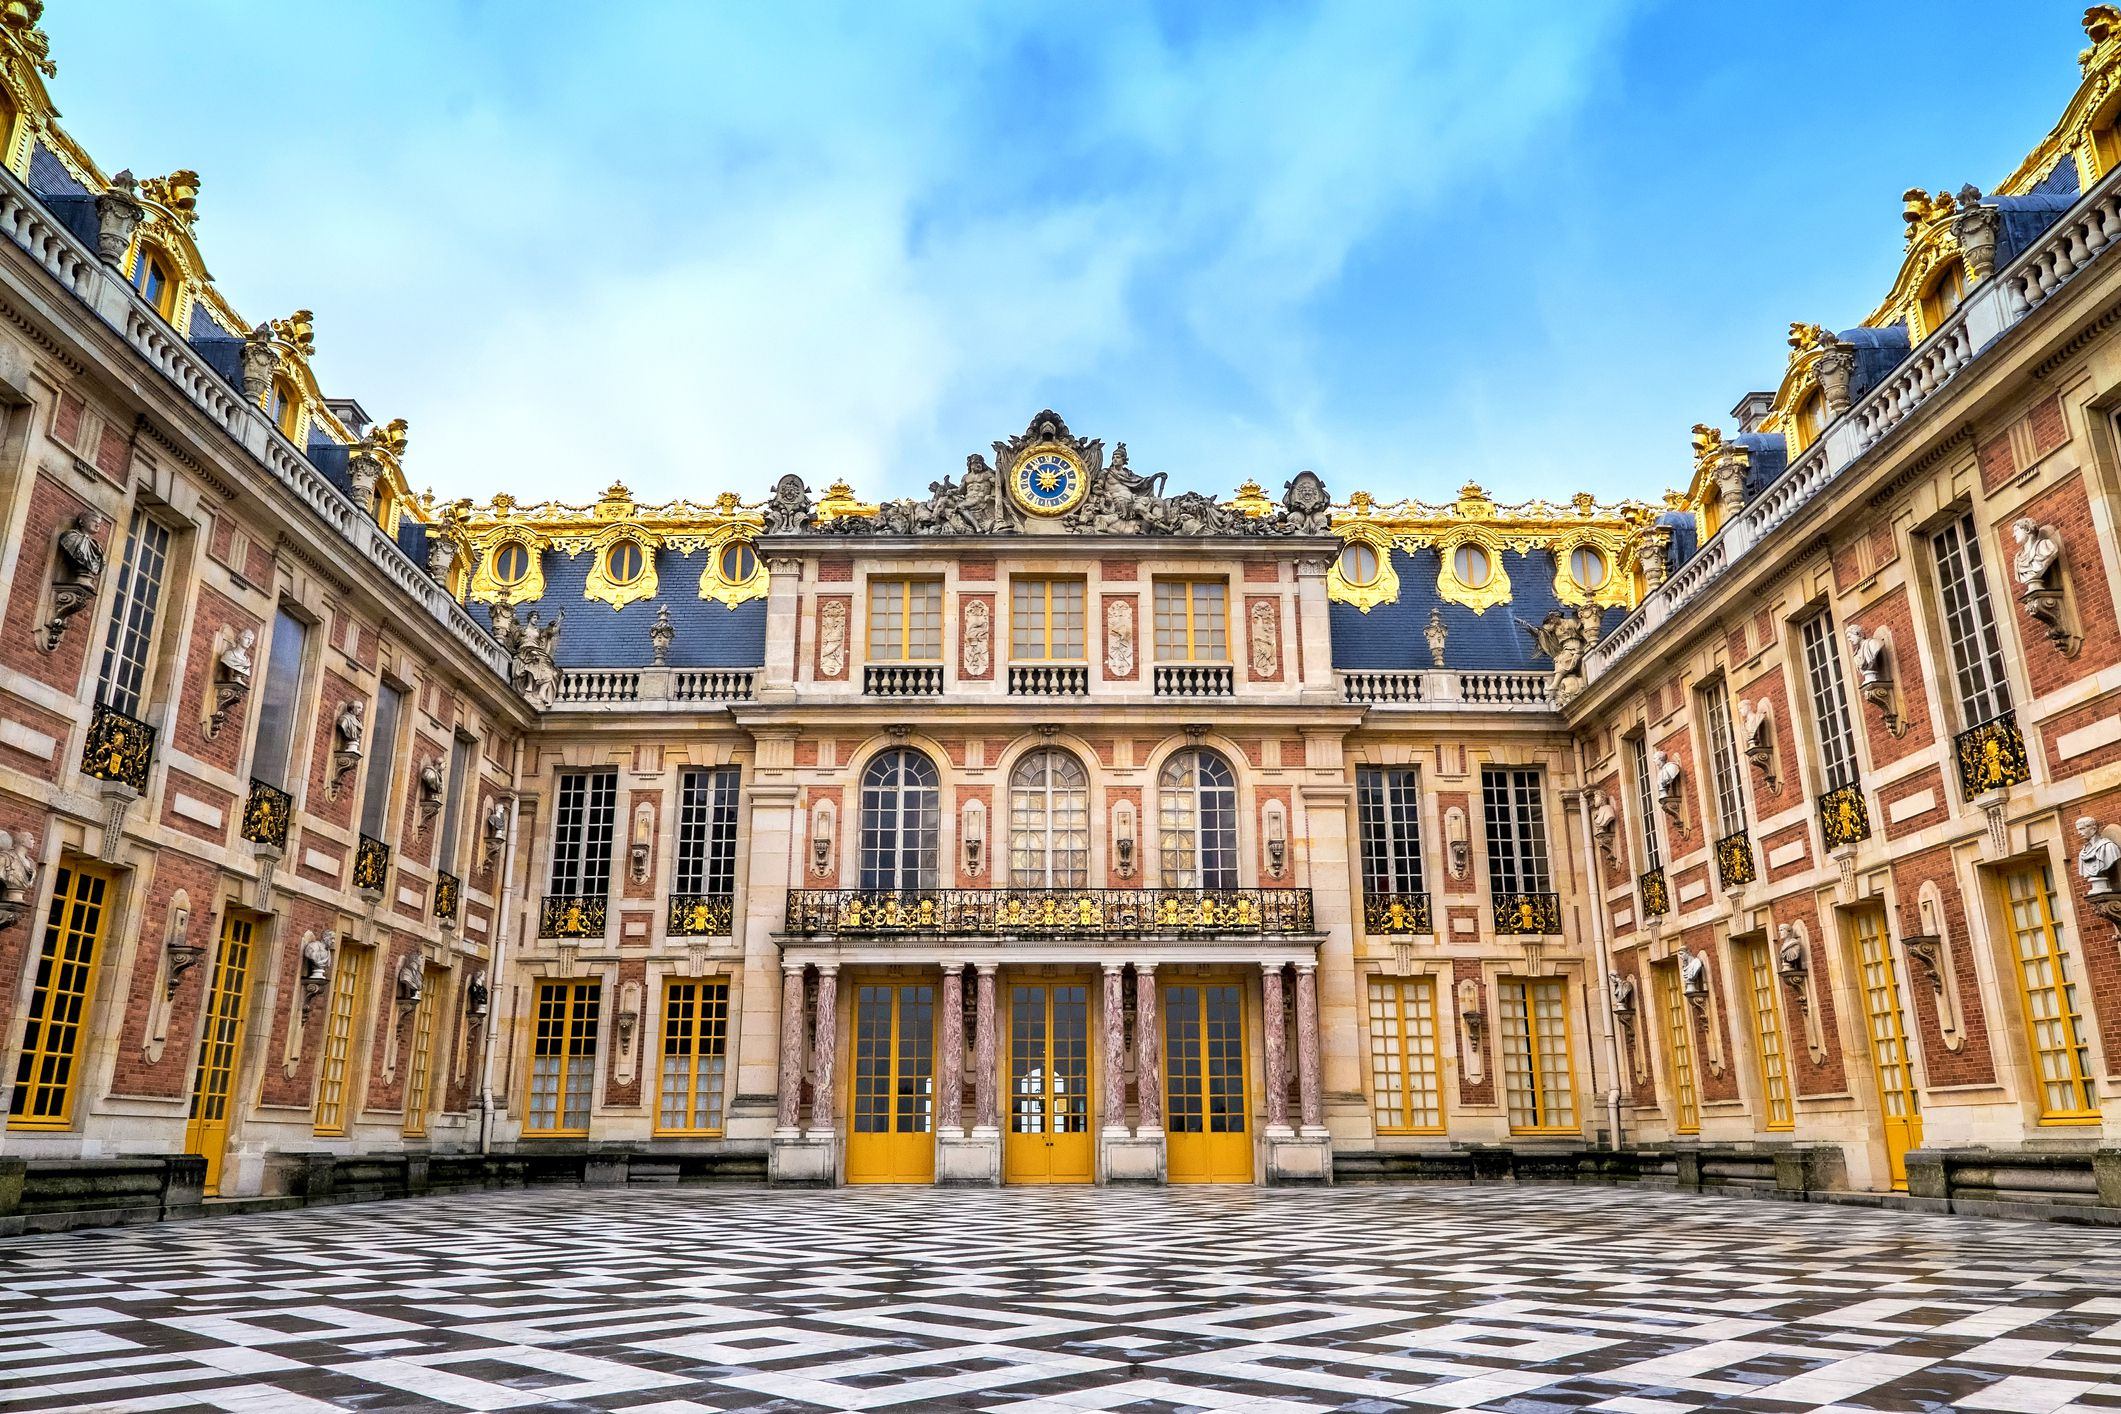
\includegraphics[scale=0.08]{versailles.jpg} \\
            Le château de Versailles
          }
          \only<9-10>{
            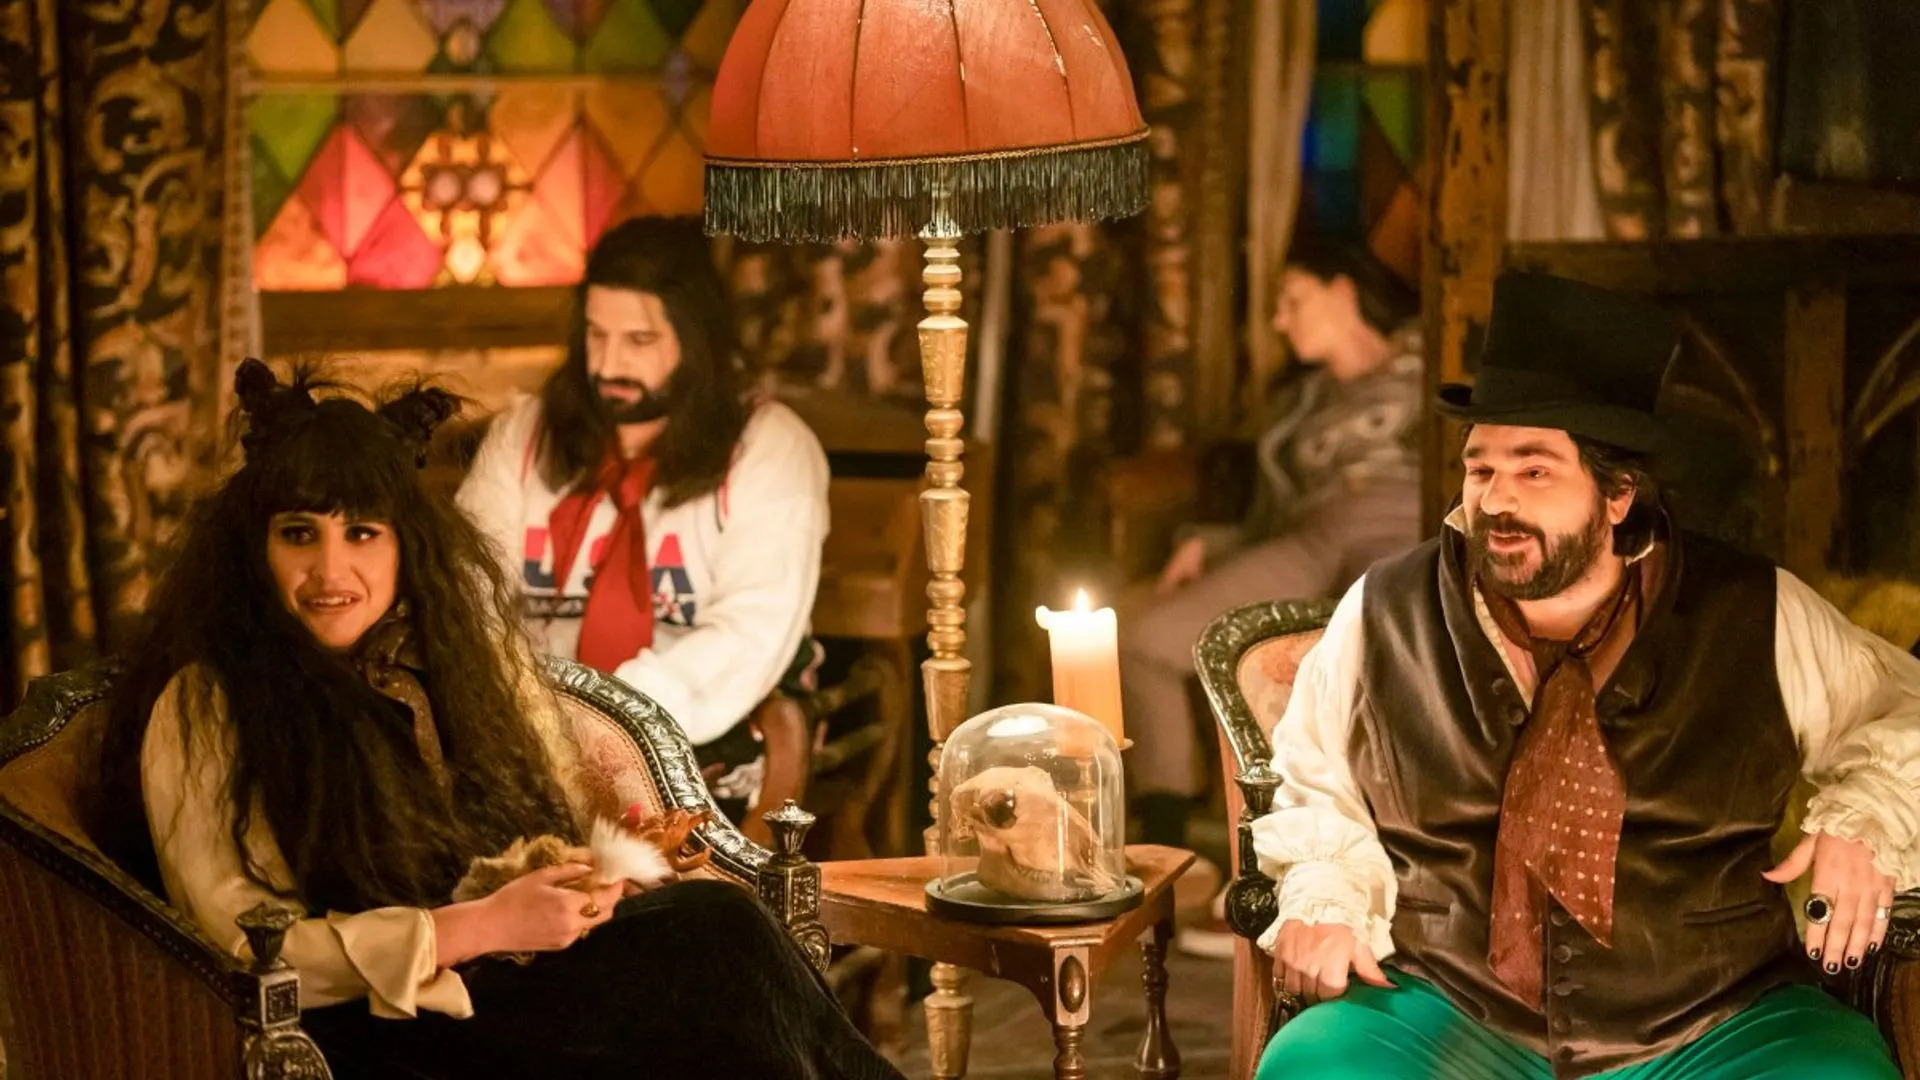
\includegraphics[scale=0.09]{amis.jpg}
          }
          \only<11-12>{
            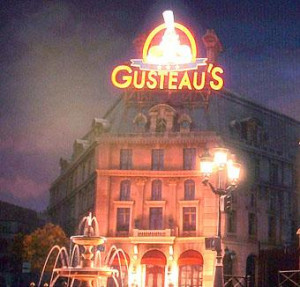
\includegraphics[scale=0.7]{gusteau.jpg}
          }
        \end{center}
      \end{minipage}
  \end{columns}
\end{frame}